\documentclass{beamer}
\usepackage[latin1]{inputenc}
\usepackage{graphicx}
\usepackage{subfigure}

\usetheme{Warsaw}
\setbeamertemplate{navigation symbols}{}

\title[SDWB\hspace{2em}\insertframenumber/ \inserttotalframenumber]{The Self-Describing Wishbone Bus (SDWB)}
\author{Manohar Vanga}
\institute{BE-CO-HT, CERN, Geneva}
\date{Jule 13, 2007}
\begin{document}

\begin{frame}
\titlepage
\end{frame}

%\tableofcontents[currentsection,currentsubsection]
%
%\AtBeginSubsection[]
%{
%  \begin{frame}<beamer>
%    \frametitle{Layout}
%    \tableofcontents[currentsection,currentsubsection]
%  \end{frame}
%}

\section{Introduction}
\subsection{Introduction}
\begin{frame}{About}
  \begin{itemize}
    \pause \item Indian\pause, studying in Spain\pause, working in Switzerland (CERN)\pause, living in France
    \pause \item Hardware \& Timing section (Beam Controls group) @ CERN
    \pause \item Develop timing \& data acquisition hardware for big toys
      \begin{itemize}
        \item Open Hardware Repository (http://ohwr.org)
      \end{itemize}
    \pause \item VME and PCI hardware (FPGA based)
    \pause \item I work on Linux device drivers
  \end{itemize}
\end{frame}

\subsection{The Hardware}
\begin{frame}{FPGAs}
  \begin{itemize}
    \pause \item Field-Programmable Gate Arrays%: can be programmed 'in the field'
    \pause \item Made up of 'logic blocks' %that can behave as simple gates up to complex combinational functions
    \pause \item Logic described in a Hardware Description Language (HDL)
    \pause \item Synthesized
    \pause \item Loaded into FPGA
    \pause \item Dynamic hardware logic!
  \end{itemize}
\end{frame}

\begin{frame}{FPGA Hardware at CERN}
\begin{figure}
\begin{center}
\subfigure[SPEC Board]
{
        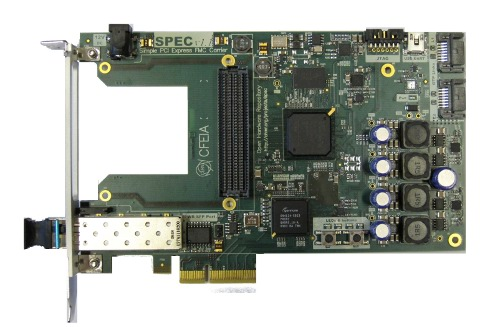
\includegraphics[width=0.4\textwidth]{spec.jpg}
}
\hspace{0.3in}
\subfigure[White Rabbit Switch]
{
        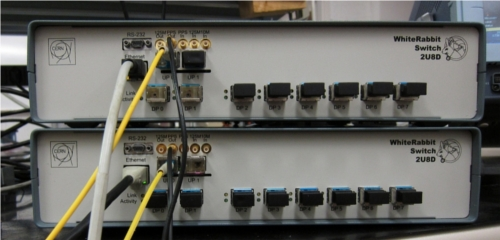
\includegraphics[width=0.4\textwidth]{wr.jpg}
}
\caption{Open Hardware from OHWR}
\label{fig1}
\end{center}
\end{figure}
\end{frame}

\begin{frame}{Wishbone Bus}
  \begin{itemize}
    \item Community-developed open bus protocol
    \pause \item Great for connecting logic blocks %within FPGA's
      \begin{itemize}
        \pause \item OpenCores (http://opencores.org)
      \end{itemize}
    \pause \item Integrator places logic blocks in Wishbone address space
    \pause \item Mapped and accessed as usual
  \end{itemize}
\end{frame}

\subsection{Device Drivers}
\begin{frame}{Device Driver Model}
  \begin{itemize}
    \item Monolithic driver? % Firmware
      \begin{itemize}
        \pause \item Modular Hardware + FPGA = Extremely vast problem space
      \end{itemize}
    \pause \item Blocks reused in different designs
      \begin{itemize}
        \pause \item Should be exploited
      \end{itemize}
%    \pause \item So we can just write drivers for specific blocks and save a lot of effort
    \pause \item Clean design: Bus auto-discovery
      \begin{itemize}
        \pause \item Not defined in the Wishbone specification
        \pause \item Let's add one!
      \end{itemize}
  \end{itemize}
\end{frame}

\subsection{Self-Describing Wishbone Bus (SDWB)}
\begin{frame}{Requirements}
  \begin{itemize}
    \item So you want to auto-discover a bus?
    \pause \item Device identification
    \pause \item Firmware metadata if possible
    \pause \item Support for device hierarchy
      \begin{itemize}
        \pause \item eg. 'Router block' controls multiple 'Ethernet port blocks'
      \end{itemize}
    \pause \item Shouldn't leave proprietary blocks out in the cold
      \begin{itemize}
        \pause \item Cannot be modified
	\pause \item Can contain entire device hierarchy
      \end{itemize}
    \pause \item Should try not to constrain designers/integrators
    \pause \item Should not force the use of external sources for metadata
  \end{itemize}
\end{frame}

\begin{frame}{Enabling Auto-Discovery: Part 1}
  \begin{itemize}
    \item Device identification
      \begin{itemize}
        \pause \item Each logic block gets vendor/device ID
        \pause \item 64-bit Vendor IDs
	\pause \item Vendor/Device name strings, Device flags etc.
      \end{itemize}
    \pause \item Firmware Metadata
      \begin{itemize}
        \pause \item ID block containing firmware version information
	\pause \item Header block holds pointer to ID block and to list of devices
      \end{itemize}
    \pause \item Only header block location needed
  \end{itemize}
\end{frame}

\begin{frame}{Enabling Auto-Discovery: Part 2}
  \begin{itemize}
    \item Supporting hierarchy description
      \begin{itemize}
	\pause \item Parents have a variable list of child locations
	\pause \item Modification of parent doesn't require modifying children
      \end{itemize}
    \pause \item Supporting proprietary blocks
      \begin{itemize}
        \pause \item Relative offsets
      \end{itemize}
    \pause \item Array of top level devices. Location in header % to 'discover' bus
  \end{itemize}
\end{frame}

\begin{frame}{Auto-discovery!}
  \includegraphics<1>[width=0.8\textwidth]{wb_1.png}
  \pause \includegraphics<2>[width=0.8\textwidth]{wb_2.png}
  \pause \includegraphics<3>[width=0.8\textwidth]{wb_3.png}
  \pause \includegraphics<4>[width=0.8\textwidth]{wb_4.png}
  \pause \includegraphics<5>[width=0.8\textwidth]{wb_5.png}
  \pause \includegraphics<6>[width=0.8\textwidth]{wb_6.png}
  \pause \includegraphics<7>[width=0.8\textwidth]{wb_7.png}
  \pause \includegraphics<8>[width=0.8\textwidth]{wb_8.png}
  \pause \includegraphics<9>[width=0.8\textwidth]{wb_9.png}
  \pause \includegraphics<10>[width=0.8\textwidth]{wb_10.png}
  \pause \includegraphics<11>[width=0.8\textwidth]{wb_11.png}
  \pause \includegraphics<12>[width=0.8\textwidth]{wb_12.png}
  \pause \includegraphics<13>[width=0.8\textwidth]{wb_13.png}
  \pause \includegraphics<14>[width=0.8\textwidth]{wb_14.png}
\end{frame}

\begin{frame}{Examples}
  \begin{itemize}
    \item Test drivers
      \begin{itemize}
        \pause \item Wishbone 1-wire and I2C block driver
	\pause \item ADC controller driver (SPEC board)
      \end{itemize}
  \end{itemize}
\end{frame}

\subsection{Future Work}
\begin{frame}{Development Efforts}
  \begin{itemize}
    \item Test specification with more complex hardware
    \pause \item Integrate with Wishbone standard
    \pause \item Go upstream
      \begin{itemize}
        \pause \item Provide support for older kernels
	\pause \item Drivers for specific blocks
      \end{itemize}
  \end{itemize}
\end{frame}

\begin{frame}{Thanks!}
  \begin{itemize}
    \item OHWR Page: http://www.ohwr.org/projects/fpga-config-space
  \end{itemize}
\end{frame}

\end{document}
